\documentclass{article}
\usepackage{pdfpages}

\title{Team Liza \\ Milestone 4}
\author{Sam Kim \\ Kevin Geisler \\ Michael Williamson \\ Brian Collins}
\date{1-26-12}

\begin{document}

\maketitle
\newpage

\tableofcontents

\newpage

\section{Domain Model}

The domain model did not change due to the Grasp principles.  Although some 
changes where made in the DCD, this did not require the Domain model to change.
This is because the additional classes will be used in the testcode class in the 
Domain Model.  The communication will continue to work as the diagram depicts below:

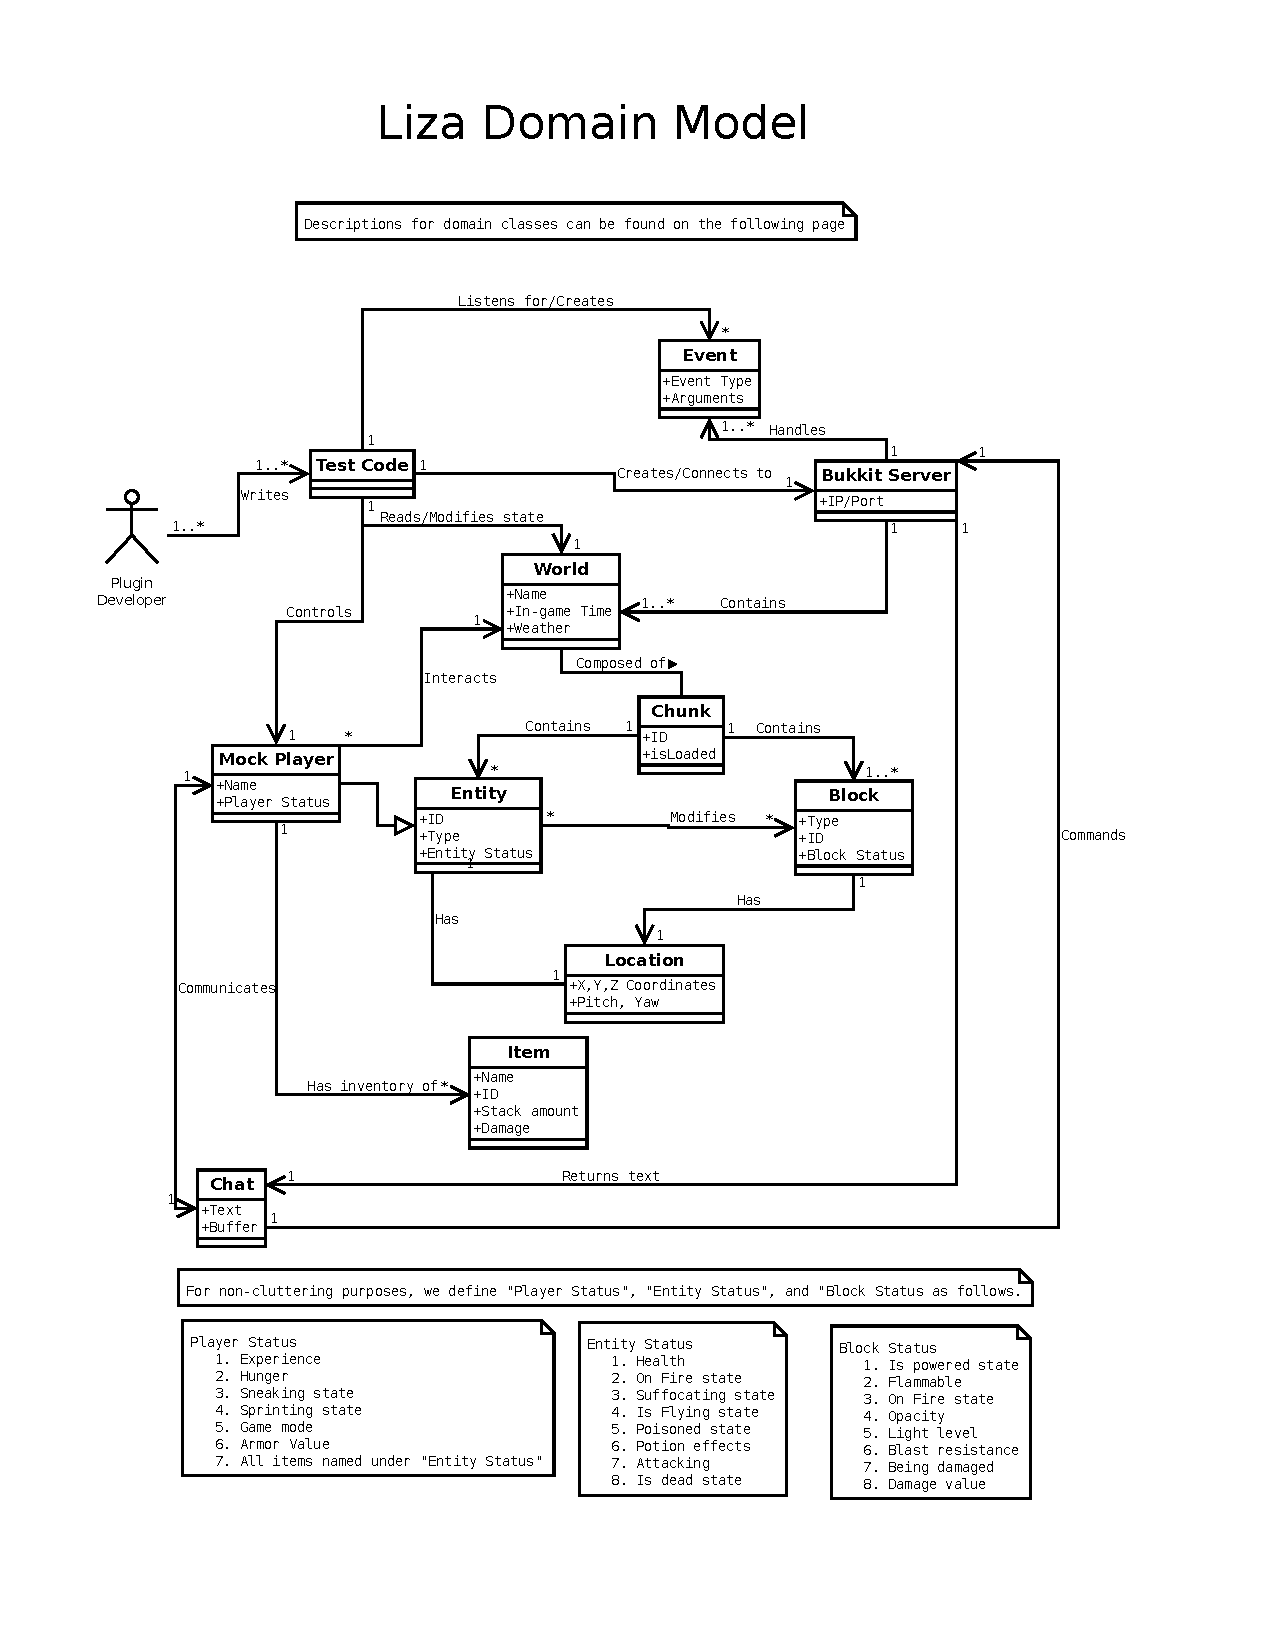
\includepdf[pages={-}]{DomainModel.pdf}



\section{System Sequence Diagrams (SSD)}

Description:  \newline

There are many SSDs that will apply to this project -- one for each assertion. 
However, each of these will follow the exact same format. Instead, we
produced a single SSD that details the flow of a test case that a developer may
write.  This includes general exception cases and alternate paths which could be
produced.  \newline 



Even though we have many SSD's in our design, most of the user interation revoles 
around the test code and the API that will be provided by the API.  Due to this, our 
general case SSD did not change.

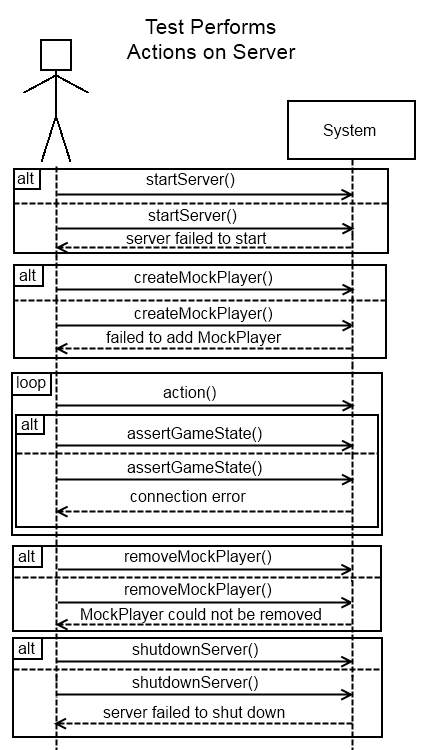
\includegraphics{ssd}

\section{Operational Contracts (OC)}

The will be a controller in Liza to startup and shutdown the server that it will control.
 Here is an operational contract which describes the startup process.:  \newline

Operation name: startServer() 
\newline \indent
Cross-References: SSD1 
\newline  \indent
Preconditions: LizaCraftController has been created.
\newline  \indent
Postconditions: CraftBukkit has been started; CraftBukkit thread has been \indent grabbed.
 \newline \newline
The shutdown operational contract is a simular process: \newline

Operation name: ShutdownServer() 
\newline \indent
Cross-References: SSD1 
\newline  \indent
Preconditions: LizaCraftController has been created; All the desired testing \indent has occured.
\newline  \indent
Postconditions: CraftBukkit has been stopped; CraftBukkit thread has been \indent stopped
 \newline \newline

\section{Package Diagram}

There exists a degree of separation between our system and Bukkit, in the
sense that our system interacts with Bukkit, yet Bukkit is not aware of our
system. However, all of the classes in our system will all belong to the same
package, due to the high amount of interaction between classes. Because
of this, a package diagram is not applicable.  However, we have included a 
diagram which depicts the relationship between Liza and Bukkit in general.
For each Bukkit class that is relavent, Liza will extend a new interface and 
create a new LizaCraft class that will implement it. \newline 

\noindent This relationship will not change due to the Grasp principles.  However, it is important to 
note that these relationships follow the protected variation design pattern.  This protects the Liza
package from the Bukkit Server.  This means that if the bukkit framework changes, that Liza will not be adversly
affected.  However, the draw back to this is that this design supports high coupling.  This taken into account there
is no way to have a separte testing framework without this effect.

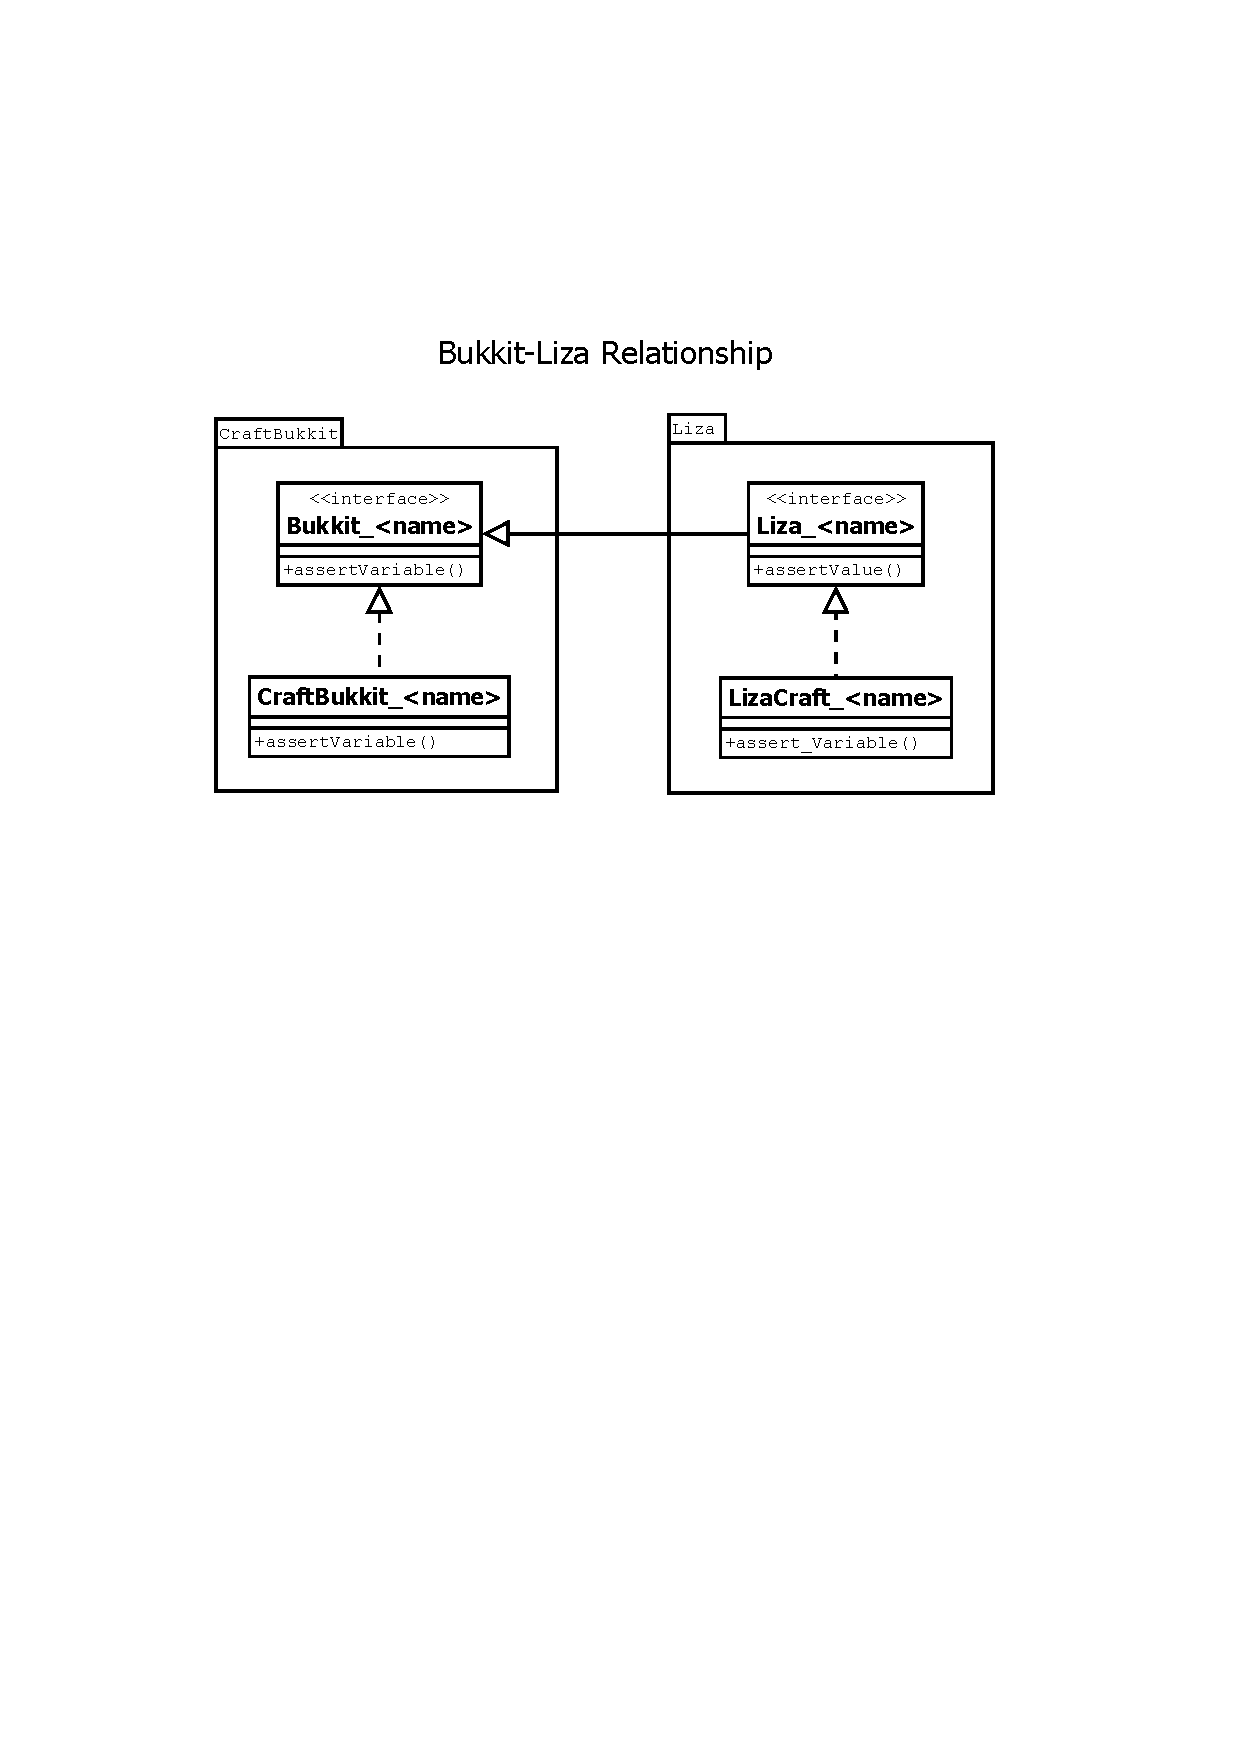
\includepdf[pages={-}]{Bukkit-Liza-Relationship.pdf}

\section{Class Diagram}

Description:
\newline

\noindent
Bukkit has two main layers: Bukkit, which is a collection of interfaces that
a plugin developer utilizes, and CraftBukkit, which is the implementation
of those interfaces. Our system will mirror this design. There is Liza, which
is a set of interfaces that inherit the Bukkit interfaces, and LizaCraft, which
is the implementation of the Liza interfaces and extends the CraftBukkit classes.
By extending the existing Bukkit and CraftBukkit, we present the API that
the developers are accustomed to, along with any new methods that may
be of use for testing, such as asserting properties. 
\newline

\noindent
There are a few new classes, however. LizaMockPlayer and its associated
implementation represent the automated player that the developer
commands. LizaMockPlayer and LizaPlayer are separated because the
latter asserts properties of any player, while the former controls only
the automated player.
\newline

\noindent
LizaListener and LizaEventExecutor handle the listening and spoofing of
events, respectively. 
\newline

\noindent
Grasp Principles:
\newline

\noindent
The Liza Unit Testing Framework follows the protected variation design pattern as
described as in the Package Diagram with the included drawback of a high cohesive system.
Due to the nature of the relationship of our system with Bukkit and Minecraft our design is limited.
With our design restriction, this limits the ability to communicate to classes without going through
other classes.  It would nice to create a more low cohesive system but we are restricted here. \newline 

\noindent
We have created a LizaCraftController following the Grasp controller principle.  This will allow for the developer 
to create one class which will create the craftserver and grab the thread of it.  At the same time the class will
contain the craftsever so that the developer will know where to go to interface with Liza.
\newline



The diagram is found on the following pages.
\newline

\newpage
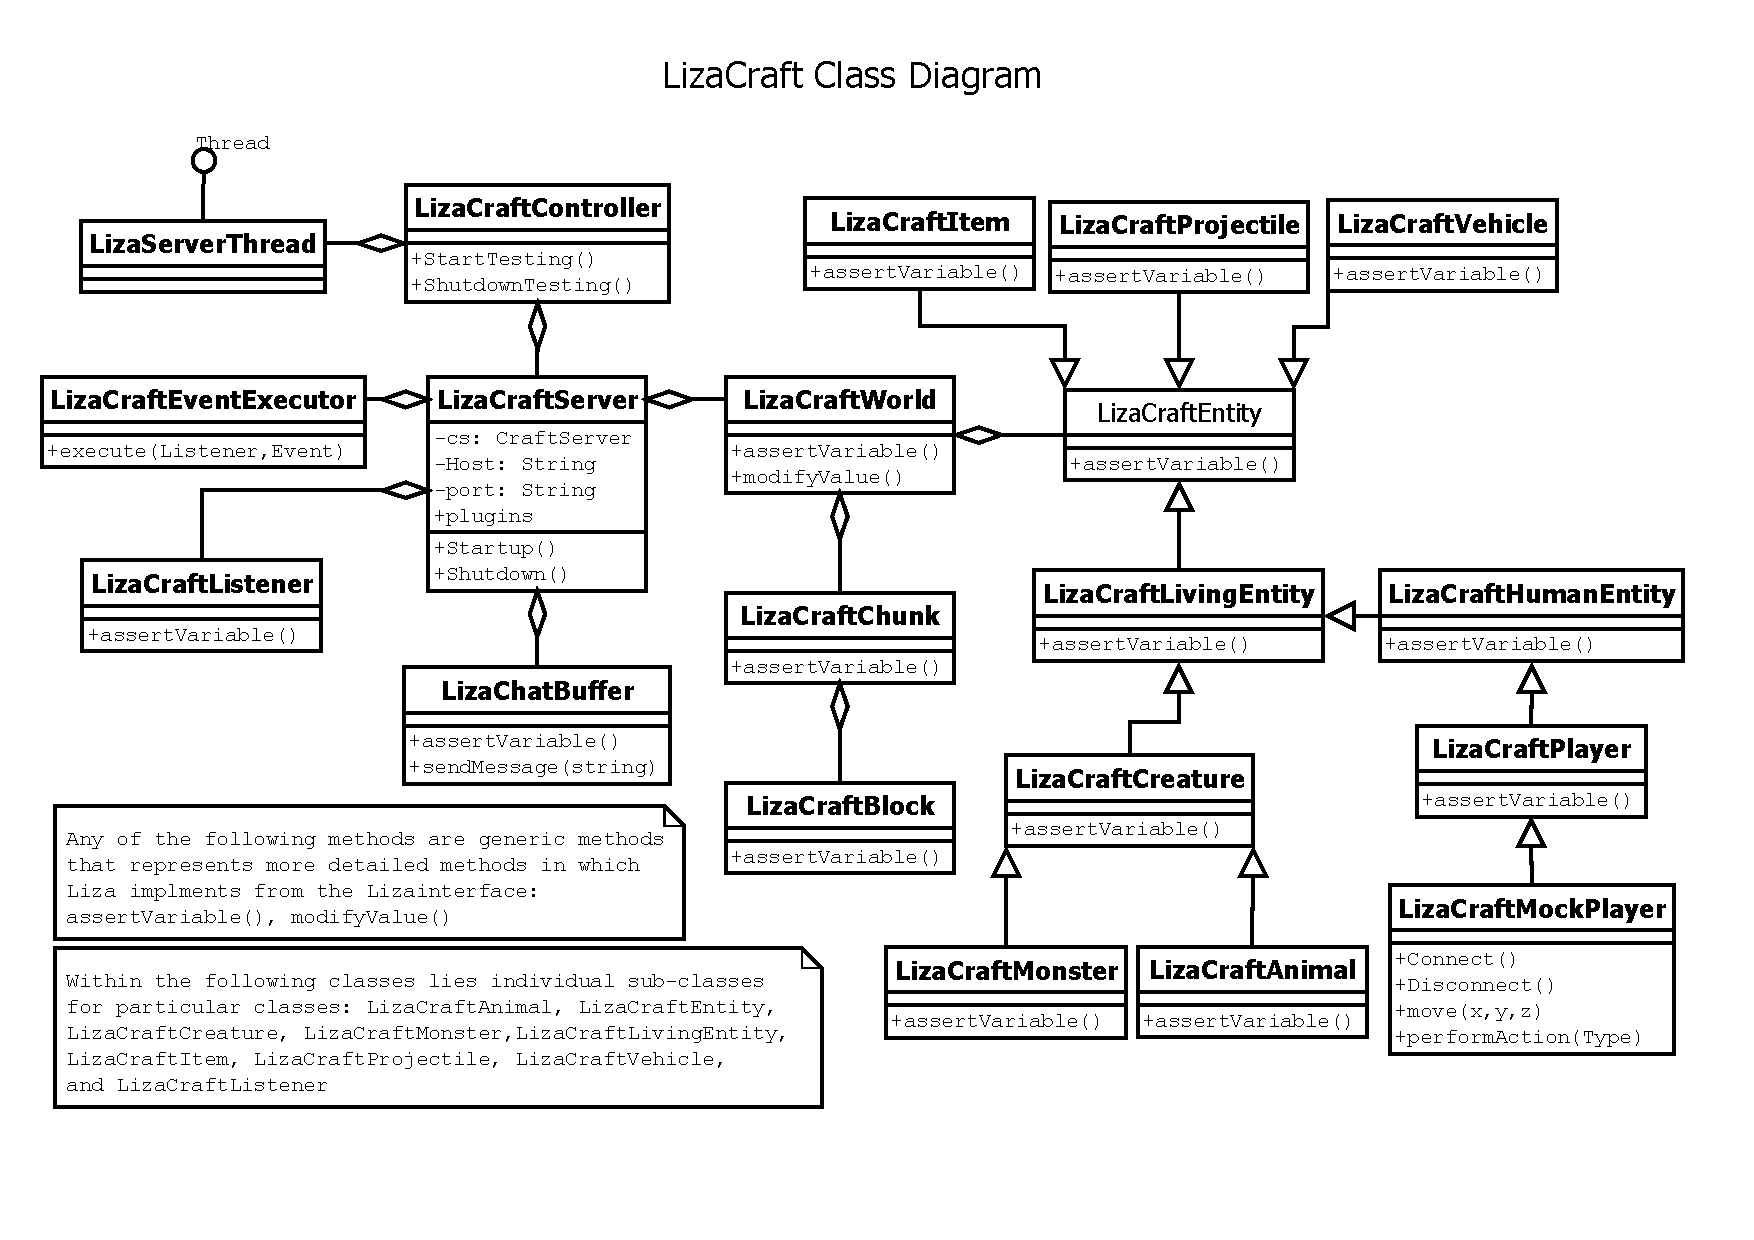
\includepdf[pages={-}]{LizaClassDiagram.pdf}

\newpage
\section{Prototype}

The prototype for this milestone is currently availble on github online at
https://github.com/geislekj/Liza

\end{document}